\section{Plan de proyecto}

\subsection{Etapas e Iteraciones}

El desarrollo del proyecto se elaborara en cuatro etapas: Elicitación, Diseño, Construcción y Transferencia. El elicitación contara con 2 iteraciones; el diseño con 3; la construcción con 4 y la transición con 2 iteraciones. Durante la etapa de elicitación se terminaran de consolidar los requerimientos funcionales y atributos de calidad de manera que queden definidos los drivers de la arquitectura. En la etapa de diseño se elaborara la especificación y modelos necesarios para comprender el funcionamiento del sistema. Durante la etapa de consturcción es implementan los modulos especificidados y en la etapa de transferencia se procede a realizar el deployment de las distintas piezas del sistema. 

La primera iteración comprenderá principalmente tareas de gestión y capacitación de los desarrolladores. Se tomó esta decisión porque identificamos varios intereses en conflicto y consideramos que es necesario establecer una prioridad entre ellos tan tempranamente como sea posible. Para hacer esto correctamente será necesario en primer lugar capacitar al equipo de desarrollo y de comunicación con los stakeholders en temas de seguridad. Priorizamos este tema en particular por haber sido considerado un atributo de calidad prioritario en el QAW y por la falta de capacitación del equipo en el mismo. 

Una vez realizada la capacitación será necesario identificar arquitecturas alternativas priorizando de manera diferente los distintos intereses en conflicto.

Contando con distintas alternativas arquitectónicas se realizará una serie de reuniones con los distintos stakeholders informándoles por qué los distintos intereses entran en conflicto desde un punto de vista tecnológico y en qué medida beneficia cada posible decisión arquitectónica a la concreción de un objetivo u otro.

Es crucial que la totalidad del equipo tenga conocimientos suficientes de seguridad para garantizar que no sean introducidas vulnerabilidades en módulos aparentemente no relacionados con el tema, por lo que la capacitación de los desarrolladores continuará y se solapará con las reuniones con los stakeholders. 

\subsubsection{Gantt}

En el primer diagrama mostramos como planeamos el proyecto a nivel general viendo así las distintas etapas y teniendo un tiempo estimado para las entregas. El tiempo estimado para
finalizar el desarrollo son 22 semanas.	

\begin{figure}[H]
 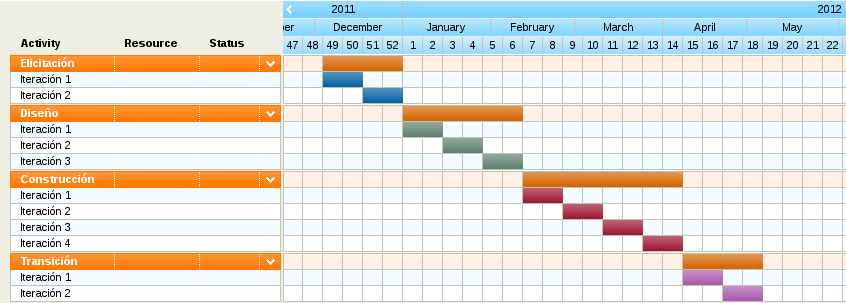
\includegraphics[scale=0.7]{./ganttetapas.png}
\end{figure}

En un segundo diagrama mostramos una de las iteraciones. Decidimos mostrar la primera iteración de la primera etapa, en donde se ven princpalmente tareas de la etapa de elicitacón. En la sección anterior comentamos de la importancia de esta etapa ya que es requerida para definir los \emph{Business Drivers} que se utilizaran para tomar decisiones en las siguientes etapas.

\begin{figure}[H]
\begin{center}
 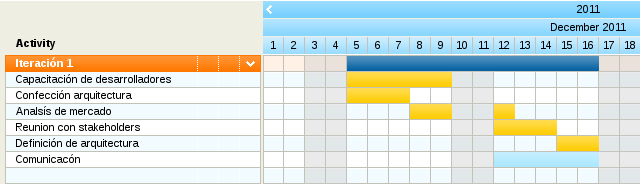
\includegraphics[scale=0.7]{./ganttiteracion.png}
\end{center}
\end{figure}

\renewcommand{\labelitemi}{$\tiny \blacksquare$}

Algunos puntos a destacar del diagrama:
\begin{itemize}
 \item Podemos ver que en esta iteración el equipo de desarrollo realizará dos tareas. Durante la primera semana se realiza la capacitación que consiste en instruir al equipo en diversos relacionados con seguridad ya que queremos minimizar problemas de este tipo. Durante la segunda semana pueden comenzar tareas de desarrollo realacionadas con los modulos relacionados a comunicación ya que se encuantra aislado al resto del sistema y tienen partes que no requieren de una arquitectura definida.
 \item El equipo de diseñadores se encarga inicialmente de realizar un arquitectura preliminar, para empezar a analizar alguno de los riesgos y problemas que nuestra arquitecutra deberá solucionar. Permite que se empiezen a analizar algunos de los problemas que se trataran con los stakeholders, y se veran que elementos externos serán requeridos.
 \item Luego habra una etapa de analisis de mercado para estar infromados de las distintas tecnologias foraneas con las que nuestro proyecto podra contar. Un punto clave para el proyecto por ejemplo es hacer un analisis de servidors y proveedores de internet, ya que debemos manter una alta disponibilidad.
 \item Por último el equipo de diseñadores se encargara de reunirse con los stakeholders para terminar de definir la arquitectura. Para esto fue necesario tener una arquitetura preliminar, y poder consensuar en las tecnologias a utilizar. 
\end{itemize}
\renewcommand{\labelitemi}{}


\subsection{Work Breakdown Structure} 

Utilizando la dinámica sugerida en las clases teóricas, generamos un WBS híbrido. En el primer nivel dividimos el sistema en 5 productos y procesos que capturan las distintas actividades a realizarse para la construcción del sistema completo. Cada uno de los productos y procesos del primer nivel agrupan funcionalidades relacionadas, excepto Actividades de gestión, que se diferencia de los demás por relacionarse con el sistema en su totalidad.

Esta división no muestra todas las dependencias entre productos y procesos, muchas de las cuales terminarán de definirse en el diagrama de Gantt de la iteración que corresponda.

Los seis elementos del primer nivel serán Interfaz, Sistema Facultad, Comunicación, Actividades de gestión, Fiscalizador y el Sistema Rectorado.

Interfaz comprende los productos y procesos relacionados con el relevamiento de requerimientos, casos de uso, codificación y prueba de la interfaz. Este producto seguramente podrá ser construído independientemente de los demás.

Sistema Facultad incluye productos y procesos orientados a la construcción del sistema autónomo de cada Facultad, que se encargará de recibir y fiscalizar la totalidad de los votos correspondientes a la misma. Los requerimientos funcionales y atributos de calidad prioritarios definitivos para este producto dependerán de varias tareas de gestión a realizarse en las primeras iteraciones, con el fin de consensuar soluciones de compromiso a los varios intereses que actualmente se encuentran en conflicto, como ser la posibilidad de contar con resultados parciales y un registro de votantes en tiempo real, en contraposición con la idea de garantizar el voto secreto.

Comunicación está conformado por productos y procesos con el fin de proveer de comunicación entre los distintos sistemas de cada Facultad. Este poducto, tal como Sistema Facultad, depende de la definición de varios aspectos de los atributos de calidad y requerimientos funcionales, por lo que dependerá de los procesos de Actividades de gestión.

Actividades de gestión reúne diversos procesos que pueden ser separados en unos pocos ejes. En primer lugar está la capacitación de los stakeholders, explicando por qué los intereses expresados entran en conflicto y cuáles alternativas arquitectónicas permiten priorizar uno u otro y en qué medida.
En segundo lugar habrán gran cantidad de procesos destinados a la validación intermedia del avance de la construcción del sistema, que consistirán en reuniones pequeñas con los principales interesados y algunas reuniones más grandes donde se muestren funcionalidades de interes general.
También habrán actividades de planificación en general, que comprenderá, por ejemplo, la confección de los diagramas de Gantt de cada iteración.
Por último será necesario capacitar al equipo en temas de seguridad, para lograr que sea tenida en cuenta en todos los niveles de desarrollo y elicitación de requerimientos. Esta capacitación será una de las primeras actividades a realizarse.

Fiscalizador es el producto que tendran los diversos partidos politicos. Nuestro sistema debera armar estos sub sistemas que permitiran que los partidos politicos se comuniquen con las facultades que deseen y además se realize el recuento de votos en forma local de manera que se logre una elección más transparente. 

Sistema Rectorado incluye los productos que el rectorado estaba interesado en tener para realizar diversas tareas de gestión. Una de esas tareas era tener concimiento de los usarios que ya votaron en la elección. Además el rectorado solicitó que el sistema permita cambiar su funcionalidad para realizar plebicitos, por lo que agregamos la funcionalidad de definir las reglas de las elecciones permitiendo que sea facilmente modificable.

\begin{itemize}
 \item {\bf \emph{WBS Vox}}
\begin{itemize}
 \item {\bf Sistema Facultad}
\begin{itemize}
 \item \emph{Modulo de servicios Web} 
\begin{itemize}
 \item Se encarga de la comunicación con las distintas interfaces web.
\end{itemize}
 \item \emph{Modulo de procesamiento de votos} 
\begin{itemize}
 \item Se encarga de procesar los votos que recibe y procesarlos según las reglas enviadas por el decanato.
\end{itemize}
 \item \emph{Modulo de registro de votos} 
\begin{itemize}
 \item Se encarga registrar los votos junto con las personas que votaron.
\end{itemize}
 \item \emph{Modulo de publicador de votos} 
\begin{itemize}
 \item Se encarga de enviar a todos los fiscalizadores los votos que esta procesando.
\end{itemize}
\end{itemize}
 \item {\bf Interfaz de Usuario}
\begin{itemize}
 \item \emph{Modulo de autenticación}
\begin{itemize}
 \item Se encarga de validar que el usuario es miembro del departamento
 \item {\bf Caso de uso:} Un usuario quiere ingresar al sistema
\end{itemize}
 \item \emph{Modulo de formularios de votos}
\begin{itemize}
 \item Se encarga de mostrar al usuario la lista de candidatos y darle opión de elegir
 \item {\bf Caso de uso:} Un usuario quiere emitir un voto
\end{itemize}
 \item \emph{Modulo de envio de votos}
\begin{itemize}
 \item Se encarga de enviar el voto al sistema de la facultad
 \item {\bf Caso de uso:} Un usuario quiere emitir un voto
\end{itemize}
 \item \emph{Modulo de idiomas}
\begin{itemize}
 \item Se encarga de adminisitrar los idiomas soportados en la interfaz de usuario
 \item {\bf Caso de uso:} Cambio de idioma en la interfaz de usuario
\end{itemize}
\end{itemize}
 \item {\bf Comunicación}
\begin{itemize}
 \item \emph{Modulo de encriptación/desencriptación}
\begin{itemize}
 \item Se encarga de encriptar y desencriptar la información enviada y recibida
 \item {\bf Caso de uso:} Conexión desde diversas plataformas
\end{itemize}
 \item \emph{Modulo de no repudiación}
\begin{itemize}
 \item Se encarga de verificar que las entidades que pretenden ser miembros del departamento realmente lo sean
\end{itemize}
 \item \emph{Modulo de confiabilidad de conexión}
\begin{itemize}
 \item Se encarga de controlar los canales que deben ser confiables
\end{itemize}
\end{itemize}
 \item {\bf Actividades de Gestión}
\begin{itemize}
 \item \emph{Capacitación de desarrolladores}
\begin{itemize}
 \item Se debe capacitar a los desarrolladores para que sistema implentado sea seguro
\end{itemize}
 \item \emph{Licitación de servicios y hardware}
\begin{itemize}
 \item Se debe hacer un analisis del hardware a ser utilizado y servicios externos que se utilizaran
\end{itemize}
 \item \emph{Armado de plan de proyecto}
\begin{itemize}
 \item Se debe realizar tareas de gestión relacionadas con la planificación
\end{itemize}
\end{itemize}
 \item {\bf Fiscalizadores}
\begin{itemize}
 \item \emph{Modulo de recibo de votos}
\begin{itemize}
 \item Se encarga de recibir los votos del sistema de la facultad
\end{itemize}
 \item \emph{Modulo de subscripción a facultades}
\begin{itemize}
 \item Se encarga de administrar las subscripciones a las distintas facultades
\end{itemize}
 \item \emph{Modulo de recuento de votos}
\begin{itemize}
 \item Se encarga de procesar los votos que recibe haciendo un recuento de votos
 \item {\bf Caso de uso:} Fiscalización parcial de los resultados
\end{itemize}
\end{itemize}
 \item {\bf Sistema Rectorado}
\begin{itemize}
 \item \emph{Modulo de confección de reglas}
\begin{itemize}
 \item Se encarga de definir reglas para procesar los votos
 \item {\bf Caso de uso:} El rectorado quiere enviar nuevos reglamentos a las facultades
\end{itemize}
 \item \emph{Modulo control de votantes}
\begin{itemize}
 \item Se encarga de consultar a los sistemas de las facultades quienes votaron
 \item {\bf Caso de uso:} Auditibilidad de votantes
\end{itemize}
 \item \emph{Modulo de administración de candidatos}
\begin{itemize}
 \item Se encarga de administrar a los candidatos de las distintas facultades
\end{itemize}
\end{itemize}
\end{itemize}
\end{itemize}


Para la facilitación de lectura omitimos escribir el nivel más bajo del WBS para poder ver descripciones de cada modulo. Cada uno de los modulos pueden ser divididos en diferentes procesos
los cuales serán asignados distintas horas dependiendo del producto.
\begin{itemize}
 \item Analisis funcional
 \item Diseño
 \item Codificación
 \item Elaboración de Plan de Pruebas
 \item Ejecución de Pruebas Unitarias
 \item Ejecución de Pruebas de Integración
 \item Ejecución de Pruebas de Aceptación
 \item Correción de Errores
 \item Instalación en ambiente de prueba
 \item Verificación Final
 \item Revisión de Alcance
\end{itemize}	
